\subsection{Luenberger Observer} 
\label{sec:simpleObserver}

Parallel to structural analysis method an observer based method have been designed for fault detection in magnetorquer based actuators. Here will be discussed a Luenberger-like form which is based directly on the non-linear dynamics. In previous chapter has been discussed that for each axis there is a pair of magnetorquers. The redundant magnetic actuators are used for reconfiguration in the presence of a fault or failure.\\    The Luenberger-like observer is based on the dynamic equation \ref{eq:seom} and for the sake of brevity is rewritten here as   

%
\begin{flalign}
\vec{\dot \omega}	
= 
{-\underline{I}_{s}^{-1} \underline{\omega}^\times \underline{I}_{s}\vec{\omega}-\underline{I}_{s}^{-1}\underline{\omega}^\times \vec{h_{rw}}+\underline{I}_{s}^{-1}[\vec{N_{rw}} + \vec{N_{mt}}+\vec{N_{dist}}}]
\label{eq:seom22}
\end{flalign}
%
where the time dependency of the variables has been suppressed for clarity. Rearranging the above equation and by adding the fault vector $\vec{F_{MT}}$ it can obtained 
%
\begin{flalign}
\vec{\dot \omega}	
= 
\underbrace{-\underline{I}_{s}^{-1}  [(\underline{I}_{s}\vec{\omega})^\times- (\vec{h_{rw}})^\times]}_{\underline{A}}\vec{\omega}+\underbrace{\underline{I}_{s}^{-1}}_{\underline{B}} \underbrace{[\vec{N_{rw}} + \vec{N_{mt}}]}_{\vec{u}}+\underline{I}_{s}^{-1}\vec{N_{dist}}+\vec{{F}_{MT}}
\label{eq:seom2244}
\end{flalign}
%  
where $\underline{A}=-\underline{I}_{s}^{-1}  [(\underline{I}_{s}\vec{\omega})^\times- (\vec{h_{rw}})^\times] $ is the system matrix, $ \underline{B}= \underline{I}_{s}^{-1}$ is the input matrix, $\vec{N_{actual}} =\vec{N_{rw}} + \vec{N_{mt}} $ is the input vector and $\vec{N_{dist}}= \vec{d}$ is the disturbance vector. The system can now be written in Luenberger-like form as
%
\begin{flalign}
\vec{\dot{{\hat \omega}}} = \underline{A}{\hat{{\vec{\omega}}}}+\underline{B}\vec{u}+\underline{B}\vec{d}+\underline{L}\underline{C}({\vec{\omega}}-{\hat{{\vec{\omega}}}})
\label{eq:seom255554}
\end{flalign}
% 
with $\underline{L}$ be the observer gain and the output vector can be written as
\begin{flalign}
\vec{y} = \underline{C}\hat{\vec{\omega}}
\label{eq:seom2554}
\end{flalign}
with $\underline{C}$ be identity matrix. The matrix $\underline{A}$ is found by using the maximum values of $\vec{\omega}$ and $\vec{h_{rw}}$ which were obtained by running the simulation over one period, and thus the gain matrix is obtained by pole placement as
\begin{equation}
\underline{L}  = 
\begin{bmatrix}
-3.0000       & -0.0014 &  0.0004 \\
0.0011       &-4.0000  &  -0.0163  \\
-0.0003    &  0.0163   & -5.0000
\end{bmatrix} 
\label{eq:orthoMatrix22}
\end{equation}
%
\subsubsection{Residual generation}
 %
 Assuming that the motors are fault free a residual can be generated from the Luenberger-like observer. By denoting $\vec{N_{obs}} =\vec{I_s}\vec{\dot{{\hat \omega}}}$ where $I$ is the inertia of the satellite then a residual can be generated as
 
 %
 \begin{equation}
 residual = \vec{N_{actual}} - \vec{N_{obs}}
 \label{eq:residualObs}
 \end{equation}
 %
 thus if $\lVert \vec{residual} \rVert \geq threshold$ a fault has been occurred. The structure of Luenberger-like observer can be seen in \figref{fig:obe} and the generated residual signal in \figref{fig:observerresidual} . 
 %
 \begin{figure}[H]
 	\centering
 	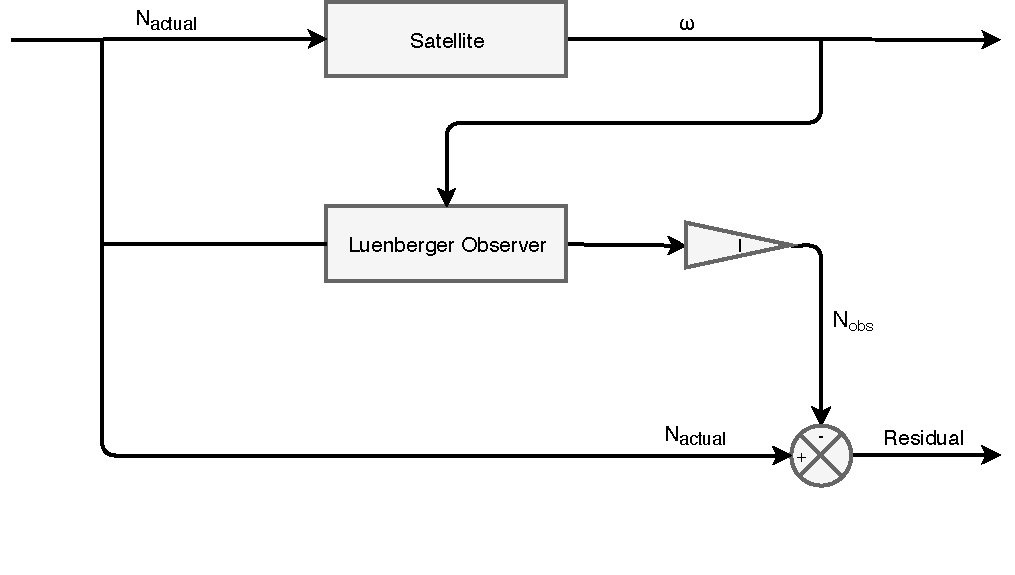
\includegraphics[width=0.7\linewidth]{figures/observerSimple}
 	\caption{Luenberger-like observer structure and residual generation}
 	\label{fig:obe}
 \end{figure}
 %
 \label{sec:simpleObserveresidual}
 %
\begin{figure}[H]
	\centering
	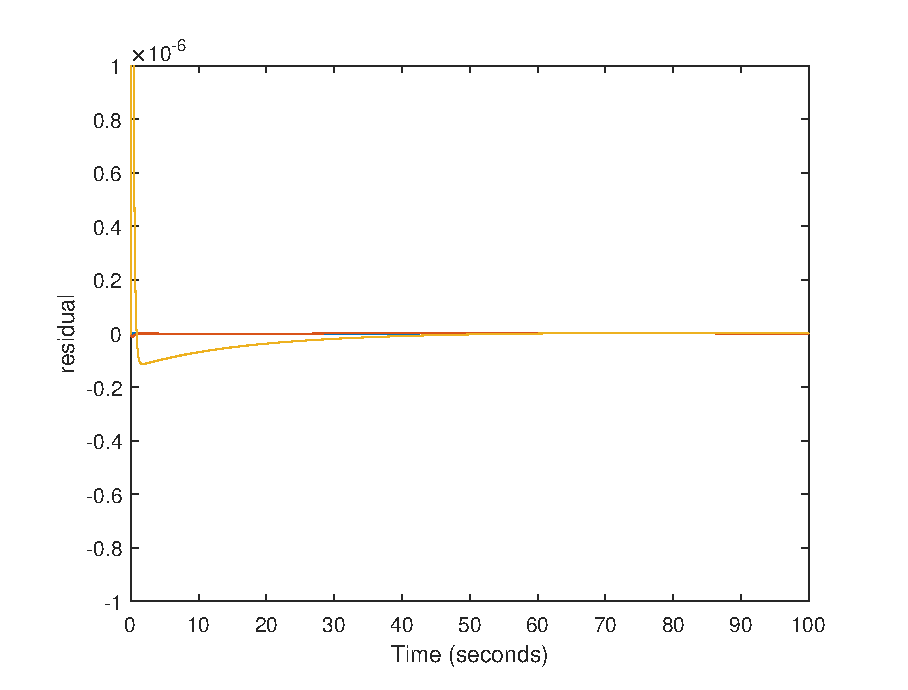
\includegraphics[width=0.7\linewidth]{figures/Observer_residual}
	\caption{Luenberger-like Observer residual signal }
	\label{fig:observerresidual}
\end{figure}
%
 Even the Luenberger-like observer is able to detect certain faults, is not robust in the sense of isolation. In order to isolate the faulty component the  Luenberger-like observer can be combined with the local structural analysis based residual which have been discussed in \ref{sec: MTStructAnal} and together by combining their flags can reconfigure the magnetorquer scheme by shutting off the faulty component and turning on the healthy one which will be discussed in chapter \ref{chap:faltHandling}. In the \figref{fig:obsflag} it can be seen the flag from the observer with a fault in the voltage supply of the first magnetorquer component at $200$[s]. 
 %
 \begin{figure}[H]
 	\centering
 	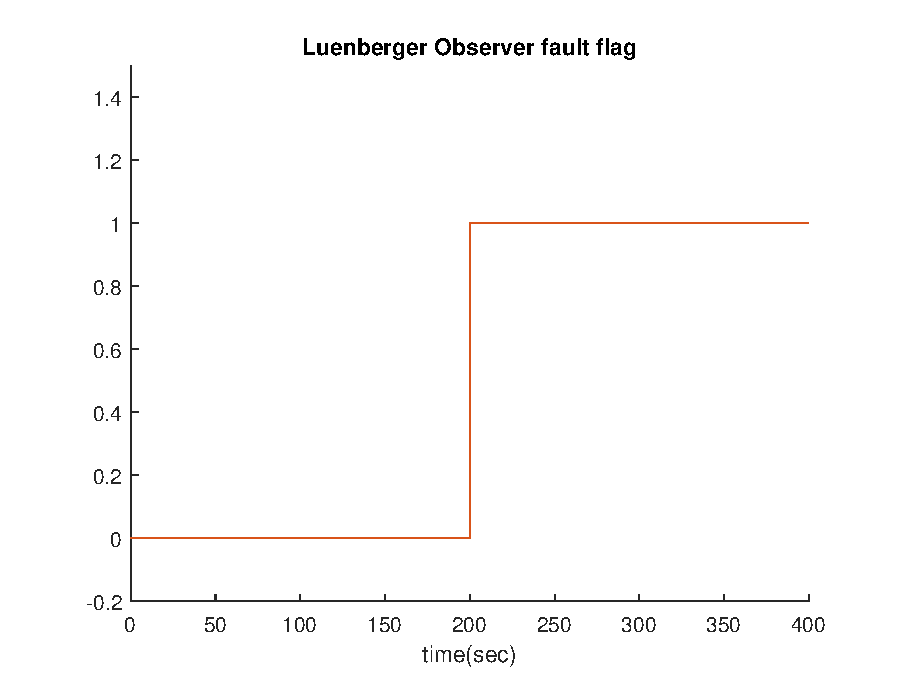
\includegraphics[width=0.7\linewidth]{figures/Luenberger_Observerflag}
 	\caption{Luenberger-like Observer flag with a fault in the voltage supply occurring at 200 seconds   }
 	\label{fig:obsflag}
 \end{figure}

%